%!TEX root = ../dissertation.tex
\begin{savequote}[75mm]
It is hard for me to empathize with an atom.
\qauthor{Dr. M. Eric Tai}
\end{savequote}

\chapter{Quantum gas microscope: \newline an overview}
\label{sec:qgm}

All experiments presented in this thesis are performed using an apparatus designed in a quantum gas microscope architecture for bosonic atoms.\footnote{Traditional microscope naming conventions typically refer to the method by which they probe the phenomena of interest (i.e. \emph{optical} microscopy, \emph{electron} microscopy). Although this microscope may seem dissimilar to this naming convention, an important point of this apparatus is that it is using the quantum properties of the degenerate atomic gas to probe physics that is harbored by Hamiltonians of interest. While I do not think this name was intentionally chosen to reflect this approach, I think it is a surprisingly appropriate/accurate description.} We conduct all experiments with a degenerate, quantum gas of $^{87}$Rb atoms in either one or two spatial dimensions by confining the atoms to a single-plane in a three-dimensional optical lattice. This single-plane of ultracold atoms lies at the focus of an imaging system with a high numerical aperture (NA) of 0.8. The occupation of these lattice sites can be read out with single-site resolution via an in-situ fluorescence imaging technique. A far more detailed description of this apparatus is provided in a number of other theses and publications \cite{Gillen2009, Peng2010, Bakr2011, Ma2014, Preiss2015, Zupancic2016, Tai2017Th, Lukin2018Th} and only the core components necessary to explain the successive work of this thesis will be explained here. 

\begin{figure}[t!]
		\includegraphics[width=\columnwidth]{figures/ch2/QGM/imaging_system_green_v2.pdf} 
		\caption{\textbf{Schematic of microscope objective, glass cell, and imaging. a)} The heart of the quantum gas microscope revolves around the combined high-NA (0.8) microscope objective built constructed from an out of vacuum objective (0.55 NA) and an in-vacuum hemispherical lens. The gas is trapped in a single plane of an optical lattice approximately $9.2\mathrm{\mu m}$ below a super-polished glass substrate. This substrate and all surrounding glass cell surfaces have no optical coatings. \textbf{b)} This example of a single-site fluorescence image of the atoms in the optical lattice displays the size of the atomic cloud that can be seen by the camera with its current magnification. The zoomed in inset demonstrates the ability to resolve the occupation of single lattice sites. Their approximate spacing is given by the lattice constant $a\sim680 \mathrm{nm}$.}
		\label{fig:qgm}	
\end{figure}

While all ultracold atom machines are an amalgamation of many parts that collectively record the successes of atomic physics for the past several decades, the schematic in Fig.~\ref{fig:qgm} only represents the latest addition and the heart of the microscopic access in this experimental apparatus. This schematic shows the high-NA imaging objective that sits outside an evacuated glass cell in which the degenerate quantum gas is formed. The custom objective that sits outside the glass cell has an NA $\approx 0.55$. The in-vacuum hemispherical lens is made of fused silica with a refractive index of $n=1.45$ and increases the combined NA to $\approx 0.8$. We create a Bose-Einstein condensate (BEC) of $^{87}$Rb by conventional evaporation in a magnetic trap in the glass cell. The BEC is then transported to the focus of this imaging system which is $\approx 10\mathrm{\mu m}$ below the bottom surface of the hemisphere. The $z$-confining lattices enter into the glass cell from the sides while the $x$-$y$ plane lattices are projected through the objective itself (Fig.~\ref{fig:qgm_latt}). The occupations of the lattice sites are imaged onto an EMCCD camera (Ixon X-3313) using fluorescence imaging from polarization gradient cooling via optical molasses beams. These two paths are the two generic options for optical access to the atoms and all other beams are combined onto these paths by either beam-splitters or dichroic filters.

\begin{figure}[t!]
		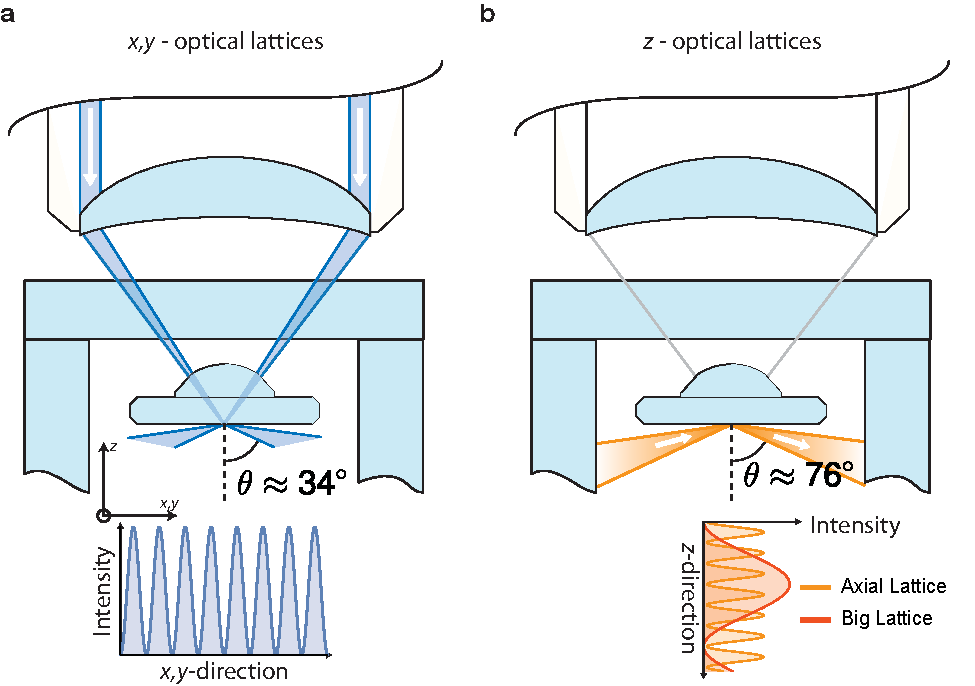
\includegraphics[width=\columnwidth]{figures/ch2/QGM/qgm_microscope_xylat_v2.pdf} 
		\caption{\textbf{Optical lattices and optical access. a)} The $x,y$-optical lattices are projected onto the atoms through the microscope objective. Both directions, $x$ and $y$, are imaged onto the atoms from their own separate phase holograms. Since these beams are not generated by retro-reflection, both their wavelength ($\lambda \approx 758\mathrm{nm}$) and their angle of incidence $\theta \approx 34^\circ$ determine the lattice spacing $a\approx 680\mathrm{nm}$. \textbf{b)} The $z$-confining lattice is produced by reflecting a single beam off the bottom of the super-polished substrate at a steep angle. Since the beam is not retro-reflected, it only produces a standing wave along the $z$-direction. There are actually two different lattice spacings created in this configuration by changing the angle of incidence. The large spacing lattice, termed the ``big" lattice, has a spacing of $\approx 9.2\mathrm{\mu m}$ to match the magnetic trap position holding the BEC. This BEC is then compressed by turning on the tighter latticed, termed the ``axial" lattice which has a spacing of $\approx 1.5 \mathrm{\mu m}$. All the optical lattice potentials in this setup are produced by spectrally broad light ($\approx 3\mathrm{nm}$). This is possible for the $x,y$-lattices since they are imaged onto the atoms. The $z$-lattices still have relatively high contrast due to the high-reflection coefficient at such steep angles and since the lattice planes are well within the coherence length ($\approx 100\mathrm{\mu m}$).}
		\label{fig:qgm_latt}	
\end{figure}

\section{Optical lattice potentials}

The dominant potential landscape experienced by the atoms is defined by optical lattices in three dimensions. The atoms are loaded from the BEC in a magnetic trap into a single two-dimension plane by being confined by a single node of a vertical ($z$-direction) lattice. All studied physics relating to the Bose-Hubbard model derived in the previous chapter is restricted to within this two-dimension plane ($x,y$-directions). All lattices are formed by interfering two beams along a given axis which produces a square lattice in all directions with a sinusoidal shape.

Nearly all optical potentials in the setup are regulated by sampling the beam intensity with a photodiode with a logarithmic amplifier (AD$8304$) which is set to $\sim 0.5\text{V/decade}$. This has two important effects in the system: i) the logarithmic amplification of the photodiode signal provides a wide dynamic range which is useful for alignment procedures, and ii) that all optical intensity ramps shown in any of the documented experimental sequences refer to how this photodiode voltage is changed. This means that a ``linear" ramp seen by the PID that regulates the optical power in a beam to the photodiode output results in an exponential ramp seen by the atoms. This is compensated in some sequences by logarithmic ramps, although often such an exponential ramp is desirable since the most sensitive Bose-Hubbard parameter, the tunneling element $J$, also scales exponentially with the lattice depth.

\subsection{$z$-Lattices}
\label{sec:zlatt}

The loading of the BEC into a single node of the $z$-confining lattices is performed by a two-step process and requires two different $z$-lattices. Both of these lattices are generated from a single beam that is reflected off the uncoated, flat surface of the hemispherical, in-vacuum lens as shown in Fig.~\ref{fig:qgm_latt}. 

The first step comes from a beam illuminating this surface from a very shallow angle and forms a large spacing lattice with a lattice constant of $\approx 9.2 \mathrm{\mu m}$ which corresponds to a recoil energy $\mathrm{E_r} \approx 2 \pi \times 7 \mathrm{Hz}$. This large spacing lattice is denoted as the ``big" lattice. The atoms are loaded into the $1^{st}$ minimum of the lattice away from the surface of the glass surface, which provides the reference for defining all $z$-positions in the apparatus. While this bottom surface is uncoated, the angle is sufficiently shallow ($\approx 88^\circ$ from normal) such that the Fresnel intensity reflection coefficient is reasonably large ($R_s\approx 0.85$). This reflection coefficient produces a lattice with a contrast $\left ( \frac{2 \sqrt{R_s}}{1 + R_s}\right )$ of $\approx 0.997$. This means that for a measured lattice depth of $V_o^{big}$, the corresponding DC offset will be $\approx 0.002 \times V_o^{big}$.

The second step involves a hand-off with a second beam that illuminates the surface from the opposite direction at a less shallow angle ($\approx 75.6^\circ$) to produce a lattice with a smaller lattice constant of $\approx 1.5 \mathrm{\mu m}$ which corresponds to a recoil energy $\mathrm{E_r} \approx 2 \pi \times 255\mathrm{Hz}$. This smaller spacing lattice is denoted as the ``axial" lattice. The atoms lie in the $6^{th}$ minimum of this lattice which overlaps with $1^{st}$ minimum of the ``big" lattice. The uncoated surface has a more detrimental effect at this illumination angle where the Fresnel intensity reflection coefficient is significantly smaller ($R_s \approx 0.39$). However, since the beam interferes with itself upon reflection, the interference contrast still remains relatively high at $\approx 0.90$. This means for a measured lattice depth of $V_o^{axial}$, the corresponding DC offset will be $\approx 0.056 \times V_o^{axial}$. The angle dependencies of both of these parameters, minimum offset and contrast, are plotted in Fig.~\ref{fig:axLatt}.

\begin{figure}[t!]
		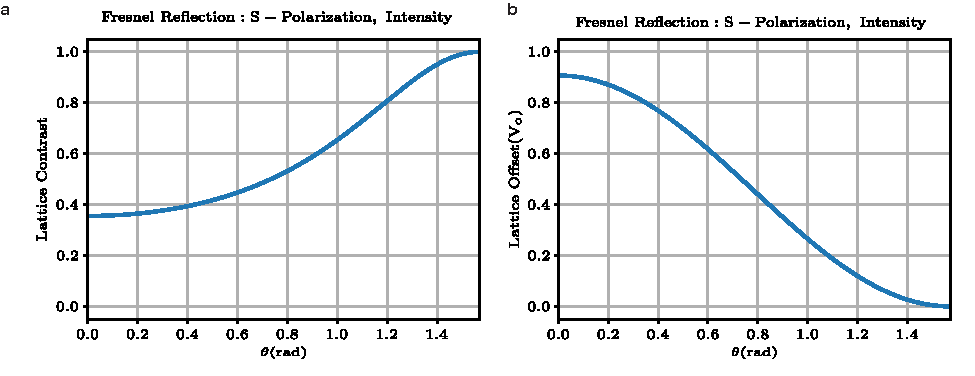
\includegraphics[width=\columnwidth]{figures/ch2/heating_rates/axLatRefv2edit.pdf} 
		\caption{\textbf{Lattice parameters vs. angle. a)} The lattice contrast, $\left ( \frac{2 \sqrt{R_s}}{1 + R_s}\right )$, plotted as a function of angle of incidence for a beam reflecting off an uncoated glass surface. The reflection coefficient is derived from the Fresnel reflection coefficient defined for intensity $R_s$. \textbf{b)} The potential energy offset incurred by non-unity reflection of a beam off an uncoated glass surface as a function of the angle of incidence. The offset is plotted as a fraction of the lattice depth seen by the atoms.}
		\label{fig:axLatt}	
\end{figure}

Both of these $z$-confining lattices are generated from an amplified Superluminescent Light Emitting Diode (SLED) source (EXALOS\textsuperscript{\textregistered} EXS$210025$-$01$) centered at $\lambda \approx 755\mathrm{nm}$. The bandwidth of this light is relatively wide $\approx 3 \mathrm{nm}$ such that the light is approximately temporally \emph{in}coherent. The corresponding coherence length is $\approx 100 \mathrm{\mu m}$ which is much longer than the $z$-lattice spacing and allows for relatively high-contrast interference quoted above. This short coherence length, while allowing the creation of a high contrast lattice at the length scales of interest, prevents interference of any of the conservative potential beams with one another or with unwanted reflections from surfaces more than $100 \mathrm{\mu m}$ away.

\subsection{$x,y$-Lattices}

In the $x$-$y$ plane, the lattices are imaged onto the atoms from a holographic mask through the objective (Fig.~\ref{fig:qgm_latt}). The spacing of this lattice is $\approx 680\mathrm{nm}$ which corresponds to a recoil energy $\mathrm{E_r} \approx 2 \pi \times 1240\mathrm{Hz}$. The holographic mask is a phase hologram that imprints a square wave of alternating $0$ and $\pi$ phase onto the profile of the illuminating beam\cite{Gillen2009,Peng2010}. This phase profile onto the beam nearly eliminates the $0^{th}$ order of the light emanating from the hologram in the far field and only the $\pm1$ orders are imaged on to the atoms. This produces a sinusoidal lattice with relatively high contrast since the imaging condition is well met by the microscope and optical setup. However, it additionally means that any unwanted artifacts (e.g. dust on the hologram) is additionally imaged onto the atom potential and creates local disorder. To alleviate some of this disorder, the beams are spatially filtered in the Fourier plane of the imaging system \cite{Peng2010}.

The same SLED source used to produce the $z$-confining lattices is also used to produce these lattices in the $x$-$y$ plane. Since the lattices are imaged onto the atoms, a more temporally incoherent source could, in principle, be used.

\subsection{Disorder (unintentional) and heating rates} \label{sec:ch2_heating}

The use of temporally incoherent light alleviates the contribution of stray reflections to unwanted interference, and hence unwanted disorder, in the system. However, since the lattices themselves are imaged from a holographic mask onto the atoms, the fidelity of the lattice potentials is very sensitive to local scatters in the image plane of the imaging system. There are two approaches to alleviate this problem: spatial filtering of the lattice beams in the Fourier plane of the system (currently implemented), or the illumination of the mask with spatially incoherent light that would average out any local scatterer.

Within the context of a faithful realization of the Bose-Hubbard model, the dominant effect from this disorder corresponds to a modulation in the on-site potential height $h_i$ in the tight-binding limit. However, the choice of blue- or red-detuned lattices affect the relationship of $h_i$ to the actual intensity of the scattered beam. In the case of red-detuned lattices, the atoms reside at the intensity maxima which means that, in the tight-binding limit, the on-site potential contains both the lattice depth $-V_o$ and the zero-point energy $\propto V_o^{1/2} \propto \hbar \omega_{ho}/2$. In a blue-detuned lattice, the atoms reside at the intensity minima and hence are sensitive to only the zero-point energy shift $\propto V_o^{1/2}$. The light used to produce the lattice potentials in the experiment has a center frequency of $\lambda=755\mathrm{nm}$ which is far blue-detuned from atomic resonances of $\lambda_{D1} = 795\mathrm{nm}$ and $\lambda_{D2}=780\mathrm{nm}$. 

%\textcolor{red}{This dependence is plotted in Fig.~\ref{fig:epsV}} as a function of scattered intensity $\epsilon$, that is now the imbalanced intensity difference between two beams interfering to produce the optical lattice (see Appendix: \ref{appendix:Ch2Cal} for derivation).

The other relevant consideration for the faithful realization of the Bose-Hubbard model in optical lattices depends on residual spontaneous scattering of light from the lattices by the atoms. This light will necessarily impart some kinetic energy onto the atom and begin to populate higher bands in the lattice. This may appear, at first glance, to not be a significant issue in the case of a blue-detuned lattice since the atoms sit at the intensity minima where there is no light to scatter. While the scattering rate is indeed significantly different for the blue- and red-detuned cases, the ``heating" rate (rate at which atomic population is moved to higher bands) is not necessarily different \cite{Pichler2010}. This result of equivalent ``heating" for both blue- and red-detuned lattices corresponds only to the increase in average energy for an atom. However, as shown in \emph{Pichler et al.}, this does not reflect the increase in entropy related to the dephasing of a many-body state evolving under the Bose-Hubbard model \cite{Pichler2010}. This will become the metric of interest and therefore the scattering rate is the more appropriate quantity for comparing between lattice detunings (Fig.~\ref{fig:heating}).

We compare several methods for calculating the spontaneous scattering rate in the lattice. The first estimate that will be considered follows an assumption of deep lattices and being deep within the Lamb-Dicke regime \cite{Grimm2000, Pichler2010}. By including the Lamb-Dicke parameter, $\eta^2=(4V_o/E_r)^{-1/2}$, the estimated heating rate for deep lattices becomes:

\begin{equation}
\gamma=E_r \frac{\Gamma}{2 \Delta} \left ( \frac{V_o}{E_r} \right )^{1/2}
\label{eqn:lambDickeEst}
\end{equation}

where $\Gamma$ is the linewidth of the D2 transition in $^{87}$Rb (nearest resonance for the blue lattice), $\Delta$ is the detuning of the lattice light from the D2 transition, and $\mathrm{E_r}$ is the lattice recoil energy. In the case of the $x$-$y$ lattices, which should have no appreciable offset, this will become a good estimate of the spontaneous scattering rate as shown in Fig.~\ref{fig:heating}. However, it is a poor description of the spontaneous scattering rate with an offset and so we take a more general approach that accounts for these DC potential offsets (\ref{eqn:sponSc}).

\begin{equation}
\gamma=E_r \frac{\Gamma}{\Delta} \int~dx~ \left ( V_{latt}(x) + V_{offset} \right ) |\psi(x)|^2
\label{eqn:sponSc}
\end{equation}

where the considered $\psi(x)$ is either the Wannier wave functions, $w_n(x)$, or the Harmonic oscillator wave functions. These more accurate estimates from (\ref{eqn:sponSc}) are plotted in Fig.~\ref{fig:heating}. The relevant lattice depths are: $\approx 2-45\mathrm{E_r}^{x,y}$ for the $x,y$ lattices, $\approx 40-250 \mathrm{E_r}^{axial}$ for the axial lattice, and $\approx 3,000-20,000 \mathrm{E_r}^{big}$ for the big lattice.

\begin{figure}[t!]
		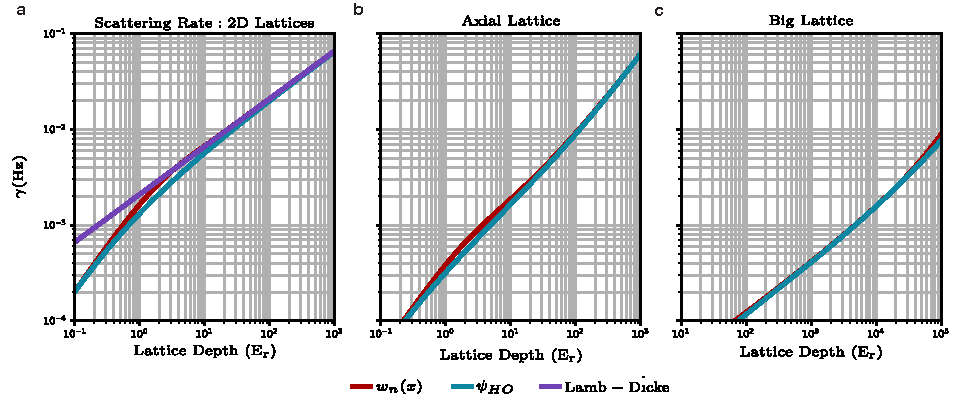
\includegraphics[width=\columnwidth]{figures/ch2/heating_rates/ScatteringRatesv2edit.pdf} 
		\caption{\textbf{Spontaneous scattering rate from optical lattices. a)} The optical lattices that provide the confinement in the $x,y$ directions have a negligible offset and can be compared in three regimes: the Harmonic oscillator wave function overlap (blue), the Wannier wave function overlap (orange), and the Lamb-Dicke approximation (green). The relevant parameter range for the physics contained in this thesis ranges from $\approx 2-45\mathrm{E_r}^{x,y}$. \textbf{b)} The spontaneous scattering from the ``axial" lattice differs from the naive Lamb-Dicke expectation due to the residual offset from imperfect reflection. The relevant parameter regime for this thesis is $\approx 40-250 \mathrm{E_r}^{axial}$. \textbf{c)} The spontaneous scattering from the ``big" lattice differs from the naive Lamb-Dicke expectation due to the residual offset from imperfect reflection. The relevant parameter regime for this thesis is $\approx 3,000-20,000 \mathrm{E_r}^{big}$.}
		\label{fig:heating}	
\end{figure}

In the case of choosing laser parameters to make optical lattices, a natural comparison for the red and blue detuned lattices can be made in the deep-lattice limit when the Lamb-Dicke regime is reached. The relationship finds the necessary detuning in a red-detuned lattice for the same scattering rate of a given blue-detuned lattice depth (given by Lamb-Dicke parameter $\eta^2$) and detuning ($\Delta_B$):

\begin{equation}
\Delta_R = \Delta_B (1+\eta^2)/\eta^2 = \Delta_B \left ( 1 + \left ( \frac{4 V_o}{E_r} \right )^{1/2} \right )
\label{eqn:detuneComp}
\end{equation}

In short, (\ref{eqn:detuneComp}) shows that a red-detuned lattice needs to be $\approx \left (1+ 2 \sqrt{V_o/E_r} \right ) \times$ more detuned than a blue-detuned lattice to obtain the same spontaneous scattering rate at a given lattice depth. While red-detuned lattices have some benefits in terms of being globally confining as an optical trap, they are often worse in terms of scattering and decoherence of the atomic system.

\section{Arbitrary potential generation}
\label{sec:ch2DMD}

The ability to realize interacting, many-body systems at ultracold temperatures in optical lattices has been the work horse of atomic gases and allows the observation of exotic physics such as the superfluid to Mott-insulator transition \cite{Greiner2002,Bloch2008,Bloch2012}. The addition of a microscope to these systems enables single-site resolution and microscopic access to the lattice sites in the system. Not only can this be used for imaging of the atoms to determine which lattice sites are occupied, but by symmetry enables the microscope to be used in reverse to project local optical potentials on the order of a lattice site.

Using this capability for single-site optical potential projection has enabled a series of pioneering experiments that allow Hamiltonian engineering on top of the bare Bose-Hubbard model. This is implemented in our apparatus via a Digital Micromirror Device (DMD) that is located in the Fourier plane of our imaging system. Even though the DMD only provides a binary mask for projecting patterns onto the atoms, the fact that it is in the Fourier plane enables finer resolution for single-site features that are spread out across a significant portion of the DMD. Only a brief description of this setup will be mentioned here such that it provides context for how it is used in the successive experiments detailed in this thesis. A more detailed description of this setup can be found in the cited articles and theses \cite{Zupancic2013,Preiss2015,Zupancic2016,Lukin2018Th}.

\begin{figure}[t!]
		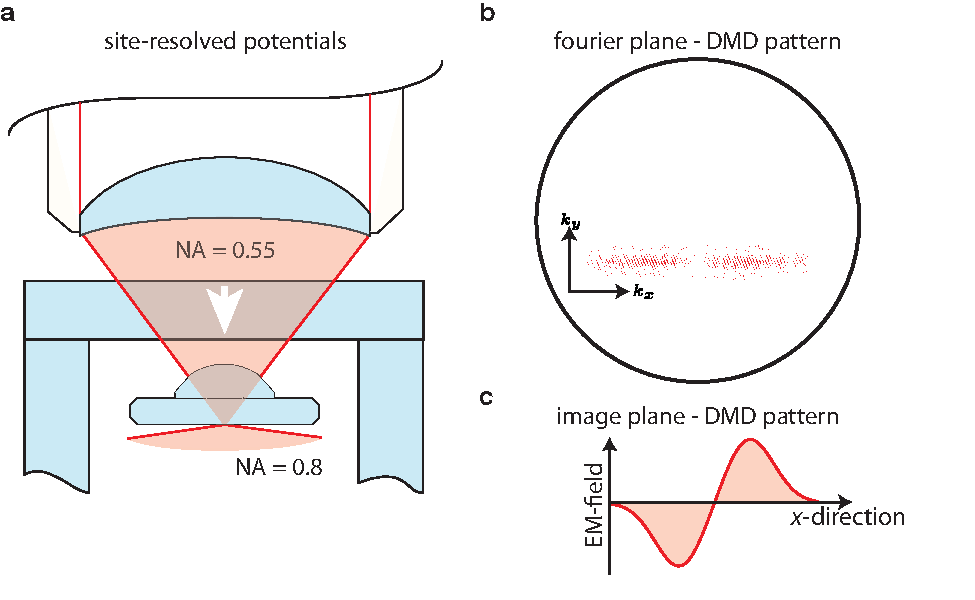
\includegraphics[width=\columnwidth]{figures/ch2/QGM/imaging_system_dmd_v2.pdf} 
		\caption{\textbf{Schematic of the DMD. a)} This schematic simply demonstrates that the arbitrary potentials created in the Fourier plane of the imaging system by the DMD are imaged through the microscope objective. \textbf{b)} This is an example of a binarized mask that is displayed by the DMD (red pixels). The underlying grating can be seen by the diagonal stripes that live within the envelope of the pattern. This pattern makes a Hermite Gaussian along one-direction ($x$-direction) and an approximate rectangular envelope along the orthogonal direction ($y$-direction). \textbf{c)} The field of the laser is what the DMD determines by the displayed binarized pattern. Here is an illustration of a through-cut of the Hermite Gaussian described in its field (rather than intensity) at the image plane where the atoms reside. Note that the atoms themselves will respond to the intensity of this pattern for all intents and purposes. This provides some degrees of freedom when actually designing a desired local potential to display on the atoms.}
		\label{fig:qgm_FP_DMD}
\end{figure}

The DMD is illuminated with a laser that is blue-detuned from the D1 and D2 transitions with a center wavelength $\lambda_{DMD} = 765~\mathrm{nm}$. By placing the DMD in the Fourier plane of the imaging system, all desired potentials must be programmed as the Fourier transform of the desired potential at the atom plane. Additionally, the potential generation on the DMD incorporates a secondary grating in the projection that allows for both amplitude and phase control of the light. Since it is really the \emph{field}\footnote{Meaning both amplitude and phase.} of the light that is tunable with the DMD, the patterns produced can be pre-compensated for aberrations in the imaging system such that the desired potentials is produced to a high fidelity. Aberrations in this system can be reduced to $\approx \lambda/10$ at the atom plane \cite{Zupancic2016,Lukin2018Th}.

\subsection{Disorder (intentional)}

The DMD is used for two primary functions for the experiments in this thesis: 1) wall-like potentials that act to isolate sections of the optical lattices and 2) the generation of local, tunable ``disorder" for the realization of localized states in the Bose-Hubbard model. For all experiments in this thesis the applied potential used to localize the wave functions is sampled from a quasi-periodic distribution of on-site potentials and will be discussed in \S \ref{sec:ch5}.

\section{Imaging and readout}

At the end of every experimental sequence, the atoms are imaged via fluorescence imaging by optical molasses beams. The recoil of this near-resonant light necessarily and significantly excites the atoms to higher-bands in the optical lattice. Even though the optical molasses light provides polarization gradient cooling to the photon recoil limit, the average energy of the atoms would not remain trapped very long in the far from resonant lattices used for studying Bose-Hubbard model physics. To keep the atoms trapped to a single lattice site during imaging we use near-resonant lattices that are blue-detuned by $\approx 55~\mathrm{GHz}$ from the $\lambda_{D1} = 795 ~\mathrm{nm}$ transition. The depth of this ``imaging" or ``pinning" lattice is $\approx 5000 ~\mathrm{E_r}$. 

During the flourescence imaging process, an additional complication occurs for multiply occupied sites. The absorption of a photon by the atom leads to the formation of an electron dipole moment with the excited state. This, in turn, induces a dipole in a nearby atom on the same lattice site such that they form an attractive molecular potential and causes the atoms to gain kinetic energy via their mutual attraction. However, the excited state will then rapidly decay and leave both atoms with enough energy to escape even the deep imaging lattice; a phenomenon that is known as photo-assisted collisions\cite{DePue1999,Bakr2009}.\footnote{Note that this effective $3$-body interaction is what allows for the photon to impart such a significant amount of energy into the atoms as kinetic energy. In a $2$-body scattering event between the atom and the photon, the atom only receives only a recoil of energy from the photon changing momentum, but not wavelength.} Importantly, this results in pair-wise loss of atoms from a lattice site during imaging such that only the parity of the on-site occupation number is imaged and is colloquially referred to as ``parity projection."

This parity projection imaging can be circumvented for one-dimensional slices of the lattice by using the DMD. The DMD is used to create two wall-like potentials that isolated a single row or column of the lattice. The corresponding lattice is then reduced in depth such that all other atoms outside of this isolated tube escape the system. Then the atoms within the isolated tube are expanded along the orthogonal direction for a brief time such that they are very spread out over the orthogonal direction during the imaging sequence\cite{Kaufman2016}. This makes it very unlikely, in a probabilistic sense, for the atoms to occupy the same site and be ejected from the lattice due to the photo-assisted collisions. This expansion allows for on-site occupation number resolution. For a one-dimensional, many-body wave function this amounts to a projective measurement onto the particle number basis or Fock basis. 

This resolution of the on-site number distribution enables several important key features for probing quantum many-body systems. It enables readout of the entire diagonal of the full system's density matrix which allows for probing correlations within this basis. It also enables higher-fidelity state readout in two ways: i) during the imaging process there is a finite probability in a densely occupied lattice, that an atom hops to a neighboring site which can result in photo-assisted collisions and appears as two ``holes" in the image that are artifacts of the imaging and not the physics being probed, and ii) it also enables post selection on total atom number which becomes paramount to quantifying atom loss during the experimental sequence. The latter is an essential tool for reducing the heating that contributes to measurements in the experiments described later on in this thesis.

\section{Calibration of energy scales}

The ability to accurately determine all experimental parameters in the system is an invaluable benefit that contributes to the precision of the results generated by this experiment. I have briefly described several of the standard calibration steps that were used ubiquitously throughout this thesis to accurately determine Bose-Hubbard parameters for conducting experiments and will not be described otherwise. Additionally, many of these methods are built upon previous results using the apparatus and in some cases are throughly detailed in those publications, which will be cited in the appropriate locations.

\subsection{Lattice depth: Kapitza-Dirac Scattering}

A particularly efficient method to calibrate the lattice depth experienced by the atoms is via Kapitza-Dirac scattering \cite{Kozuma1999,Ovchinnikov1999,Stenger1999,Gupta2001,Gadway2009}. This method requires that the atoms have Bose-condensed so that their many-body wave function has a well defined phase across the entire cloud. The lattice is then turned on very diabatically\footnote{This means the new Hamiltonian is turned on significantly faster than all the inverse energy scales in the system such the wave function itself has not evolved during the turn on time.} and illuminates the atoms for a tunable, but brief time period. This brief illumination of the atoms is such that the atoms only experience a potential that evolve the local phase of their wave function but the atoms have not had time to move yet. The imprinted phase on the atoms has a spatial structure that is proportional to the lattice potential and can be probed easily via common time of flight measurements which map the spatial Fourier components, or wavevectors of the wave function, to momentum. 

This mapping of the imprinted spatial phase on the BEC to momentum has a convenient and clean analytical form that results from the spatial phase always being commensurate with periodicity of the lattice. This results in the atomic momentum only existing at integer multiples of the lattice wavevector. The population in these integer multiples then follows the analytic form given by:

\begin{equation}
\label{eqn:KDanalytic}
P_{|\nu|}(t)= \left | \mathcal{J}_\nu \left ( \pi E_r \frac{V_o}{E_r} t \right ) \right |^2
\end{equation}
%\textcolor{red}{The derivation of this form is shown in Appendix \ref{appendix:Ch2Cal}}.
where $\mathcal{J}_\nu$ is the Bessel function of the$1^{st}$ kind, $\nu$ denotes the integer of the lattice vector and the order of the Bessel function, $V_o$ is the lattice depth in Hz, $\mathrm{E_r}$ denotes the recoil energy of the lattice, and $t$ is the time the atoms have evolved in the presence of the lattice. The evolution of the population into these modes is shown as a function of time in Fig.~\ref{fig:KDScatt}. As can be seen in this figure, the dynamics stop following the predicted evolution due to the presence of the additional trap confinement and that the wave function will also begin to redistribute atomic population in the presence of this lattice on the order of the lattice-site trap frequency $\omega_{Latt}$.

\begin{figure}[t!]
		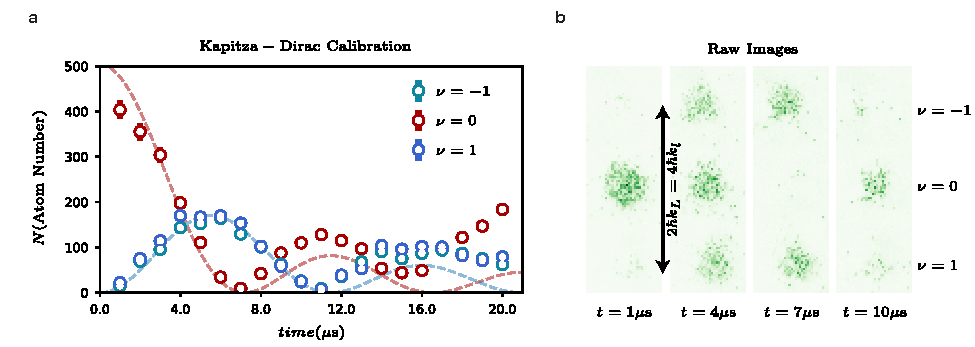
\includegraphics[width=\columnwidth]{figures/ch2/kapitza_dirac_latt_depth/KDCalv2edit.pdf} 
		\caption{\textbf{Kapitza-Dirac scattering. a)} The plotted points denote the total atom number in the various time-of-flight peaks that are separated by integer numbers of the lattice wavevector: $\nu=0$ (red), $\nu=\pm1$ (light/dark blue). The dashed lines are the fitted, analytic forms up to $\approx 10 \mathrm{\mu s}$. \textbf{b)} Example of the raw, in-situ atom images before being processed.}
		\label{fig:KDScatt}	
\end{figure}

\subsection{Tunneling $J$ : single-atom quantum walks}
\label{sec:qwcal}

The tunneling matrix element (tunneling strength), $J$, can be calibrated from the quantum walk of single atoms in one-dimensional lattices. This protocol involves first isolating a single-atom at a particular site per one-dimensional lattice. These dynamics have been explored extensively in a number of publications \cite{Hartmann2004,Lahini2012,Ahlbrecht2012,Manouchehri2014,Preiss2015} and are of significant interest in their own right. While the tunneling strength and the lattice depth have a well defined theoretical relationship that could make this calibration seem redundant, practically speaking this method provides a far more accurate estimate of the local tunneling strength.\footnote{This is partially due to some of the systematic biases in the lattice depth calibration that uses Kapitza-Dirac scattering that limit the precision of the measurement. However, the other issue is that the optical lattices used in this apparatus have local variation in disorder that can locally modify the tunneling strength $J$. Since the vast majority of experiments in this system work with appreciably large-lattice depths and small systems, this is a significant consideration for calibrating experimental parameters.} The analytic form is quite similar to the Kapitza-Dirac scattering form. The physics of the quantum walk is, in a sense, exactly complimentary to Kapitza-Dirac scattering. A single-particle which is localized in real space (completely delocalized in k-space) is evolved forward in time by unitary evolution of a new quenched Hamiltonian which has a cosine dispersion curve in k-space (real space). This necessarily realizes the same analytic result for the population of the different reciprocal orders in real space, which are now lattice sites:

\begin{equation}
\label{eqn:QWanalytic}
P_{|\nu|}(t)= \left | \mathcal{J}_\nu \left ( {2 \times 2 \pi J t} \right ) \right |^2
\end{equation}

where $\mathcal{J}_\nu$ is the Bessel function of the $1^{\text{st}}$ kind, $\nu$ denotes the integer lattice sites away from the origin and the order of the Bessel function, and $J$ is the tunneling strength. There is an additional formulation that includes the possibility for local potential gradients that can provide a better fit and is the corresponding form for what are known as Bloch oscillations:

\begin{equation}
\label{eqn:BlochOsc}
P_{|\nu|}(t)= \left | \mathcal{J}_\nu \left ( \frac{2 J}{\pi E} \sin \left( {\pi E t / h}\right ) \right ) \right |^2
\end{equation}

where $E$ is the local potential gradient. For a given evolution time $t$, a corresponding lattice size can be fit where $ |\nu| \leq L/(2 \pi J) $. \footnote{This bound is determined by the Lieb-Robinson veolocity, which for a single-atom in a lattice is determined by the steepest slope (maximum group velocity) of its corresponding band.} These fits and averaged site-occupation data are shown in Fig.~\ref{fig:QWCal}. Note that at very low-lattice depths, the tight-binding, nearest-neighbor coupled Bose-Hubbard model becomes a less accurate description of the physics in the lattice and hence higher-order tunneling terms become significant. The deviation, both theoretical and measured, is shown in Fig.~\ref{fig:QWCal}.

\begin{figure}[t!]
		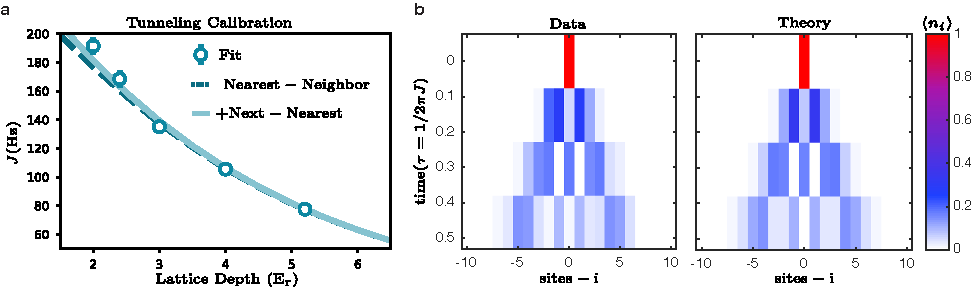
\includegraphics[width=\columnwidth ]{figures/ch2/QW_cal/qw_fit_cal_v2_edit.pdf} 
		\caption{\textbf{Quantum Walk Calibration. a)} The calibrated tunneling strength $J$ are plotted as the blue points for various measure lattice depths by fitting the time evolution of the particle's wave function to the analytical form (\ref{eqn:QWanalytic}) The analytical result for the nearest-neighbor tunneling strength $J$ as a function of lattice depth is plotted as the dashed black line. The orange line describes the expected deviation of the calibration fits to the data based upon the contributions of higher-order tunneling terms that include tunneling beyond nearest neighbors. \textbf{b)} The raw data is shown as a function of time and lattice site index $i$ for a $5.2~\mathrm{E_r}$ deep lattice. The analytical dynamics that fits best to it is shown on the right.}
		\label{fig:QWCal}	
\end{figure}

\subsection{Interaction $U$ and linear tilt $E$: photon-assisted tunneling} \label{sec:EUcal}

Determining the on-site interaction strength $U$ and local potential variation from local disorder can be determined from a single protocol that utilizes photon-assisted tunneling\cite{Ma2011}. This method first starts deep in a Mott-insulating regime where there is exactly an integer number of atoms per lattice site. Then a potential gradient is applied to the system such that it increases the on-site potential energy by $E~\mathrm{Hz/site}$ such that is larger than the interaction energy $U$. Then the lattice depth is lowered to intermediate lattice depth $\approx 15 \mathrm{E_r}$ where the tunneling $J$ is still much smaller than $U$ or $E$. The lattice depth is then sinusoidally modulated at small amplitudes at various frequencies to restore tunneling between the sites that are currently far away from resonance. When the frequency matches the energy difference between two sites, it restores tunneling and appears as strong on-site fluctuations away from the Mott-insulating state.

%\begin{figure}[t!]
%		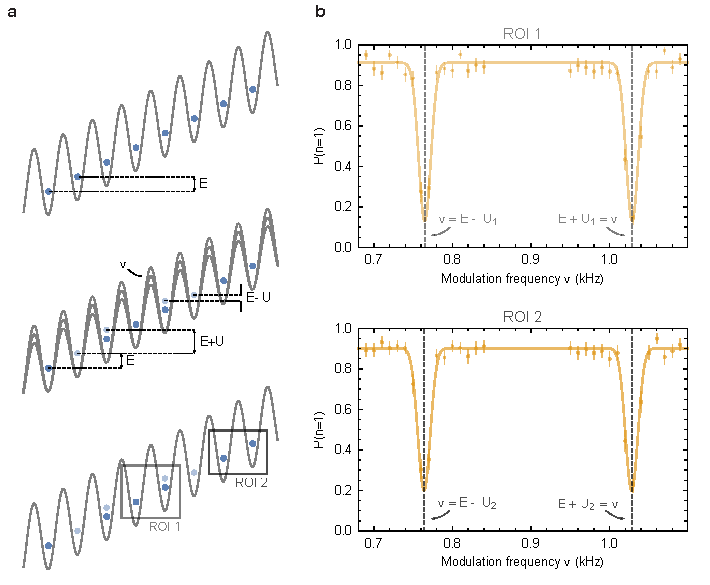
\includegraphics[width=\columnwidth]{figures/ch2/E_U_cal/UCalv2edit.pdf} 
%		\caption{\textbf{Protocol for modulation spectroscopy. a)} This illustration describes the protocol for this tilt and modulation experiment. By analyzing the system by local regions of interest (ROIs), not only can the global interaction strength be measured, but also the local variation in on-site potential offsets. \textbf{b)} Two potential ROIs are plotted as a function of the modulation frequency and the measured on-site occupancy between neighboring sites. The solid lines are fits from a two Gaussian model to extract the resonance frequencies.}
%		\label{fig:EUCal1}	
%\end{figure}

\begin{figure}
\floatbox[{\capbeside\thisfloatsetup{capbesideposition={right,top},capbesidewidth=1.5 in}}]{figure}[\FBwidth]
{\caption{\textbf{Protocol for modulation spectroscopy. a)} This illustration describes the protocol for this tilt and modulation experiment. By analyzing the system by local regions of interest (ROIs), not only can the global interaction strength be measured, but also the local variation in on-site potential offsets. \textbf{b)} Two potential ROIs are plotted as a function of the modulation frequency and the measured on-site occupancy between neighboring sites. The solid lines are fits from a two Gaussian model to extract the resonance frequencies.}
		\label{fig:EUCal1}}
{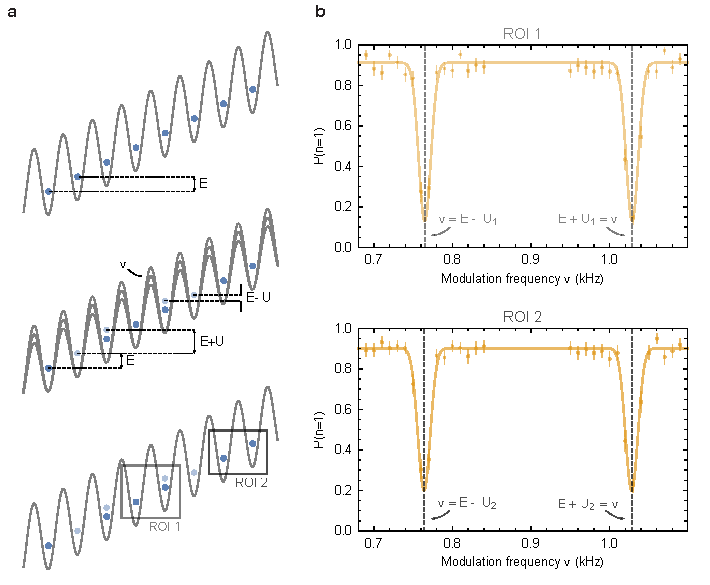
\includegraphics[width=4 in]{figures/ch2/E_U_cal/UCalv2edit.pdf} }
\end{figure}

There is a useful asymmetry in this protocol due to the on-site interactions. In the regime where $E>U$, the energy difference for an atom to hop to neighboring sites will cost either $E+U$ or $E-U$ energy depending upon the direction of increasing gradient potential. This means that by measuring out both resonance conditions both $E$ and $U$ can be calibrated locally. This is demonstrated in Fig.~\ref{fig:EUCal2} where the two resonances are measured, and the variance of the tilt $E$ and the interaction $U$ across the measured region reveal residual on-site disorder and on-site curvature. 

\begin{figure}[t!]
		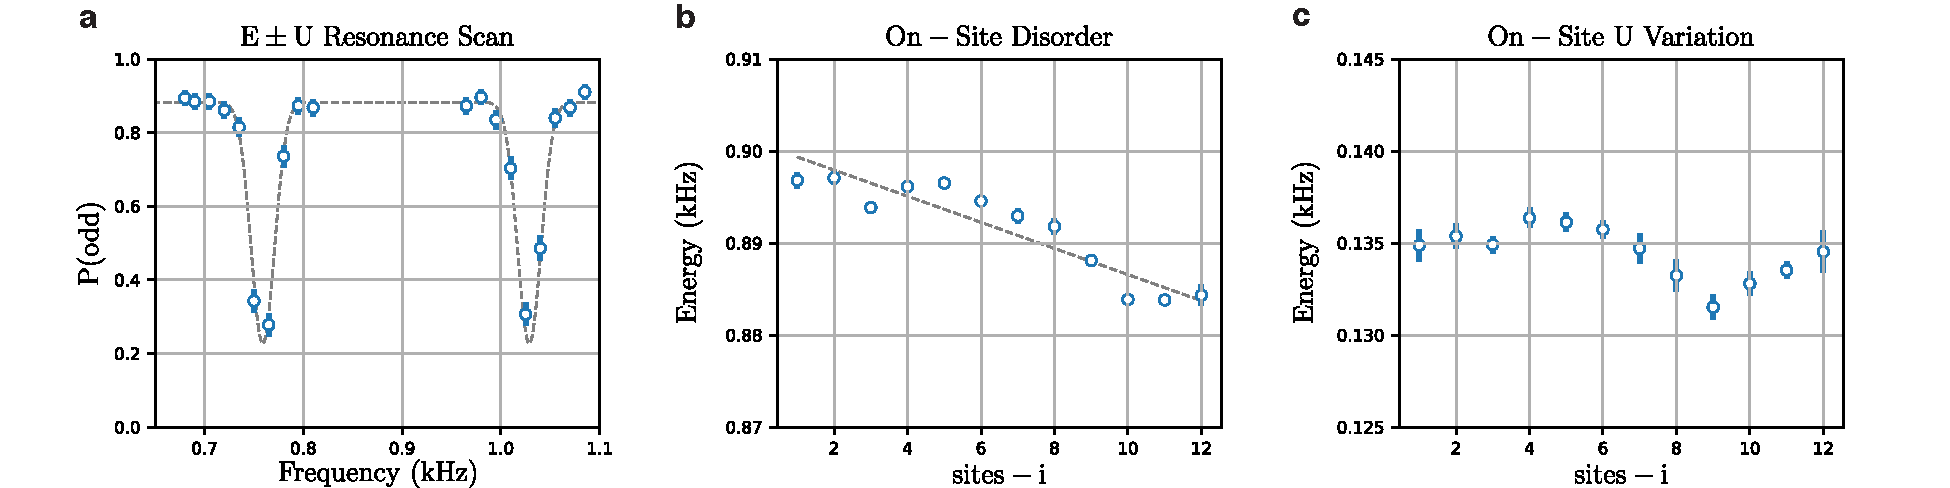
\includegraphics[width=\columnwidth]{figures/ch2/E_U_cal/EUCalv2edit.pdf} 
		\caption{\textbf{Calibration of interaction ($U$), tilt ($E$), and variation in on-site potential ($h_i$). a)} The same ROI plot as shown in Fig.~\ref{fig:EUCal1} is demonstrated for a system with the interaction strength defined by the $z$-confinement derived from the ``big" lattice. \textbf{b)} Variation of tilt as a function of the lattice site of interest. The linear fit here suggests a residual curvature of the on-site lattice offsets since it is the derivative of the on-site potential offset profile that is measured by this protocol. \textbf{c)} Variation of interaction as a function of lattice site index. Note that this varies only on the order of $1~\mathrm{Hz}$ since it is effect by the on-site variation in curvature.}
		\label{fig:EUCal2}	
\end{figure}

While the tilt $E$ here is described as purely a part of a process that is necessary to suppress tunneling such that $U$ and on-site differences can be measured, the tilt itself is also sometimes the quantity of interest. In some experimental schemes that implement synthetic magnetic fields in ultracold atom experiments, a potential gradient is used to suppress the bare, resonant tunneling in the lattice $J$ along one direction which is then restored with a spatially varying phase. This has been explored in several cold atom experiments in real space \cite{Aidelsburger2013,Miyake2013} and was implemented in this system to probe the Harper-Hofstadter model\cite{Tai2017} and is described in significant detail in the cited thesis \cite{Tai2017Th}.

\subsection{On-site potential offsets $h_i$ : adiabatic transfer}
\label{sec:DMDpotCal}

The generation of single-site resolved potentials $h_i$ are created via the DMD installed in the apparatus and are used extensively for state initialization and site-occupation readout during imaging. In both of these cases, the absolute depth of the potentials used is not particularly important since both procedures are relatively insensitive to them. However, some of the experiments in this thesis rely on a particular relationship of the on-site potential offsets $h_i$, to both the tunneling strength $J$ and interaction strength $U$. By calibrating these potential offsets using the atoms we can both compare how precisely the DMD can produce a desired optical potential and the absolute height of these potentials in Hz.


%\begin{figure}[t!]
%		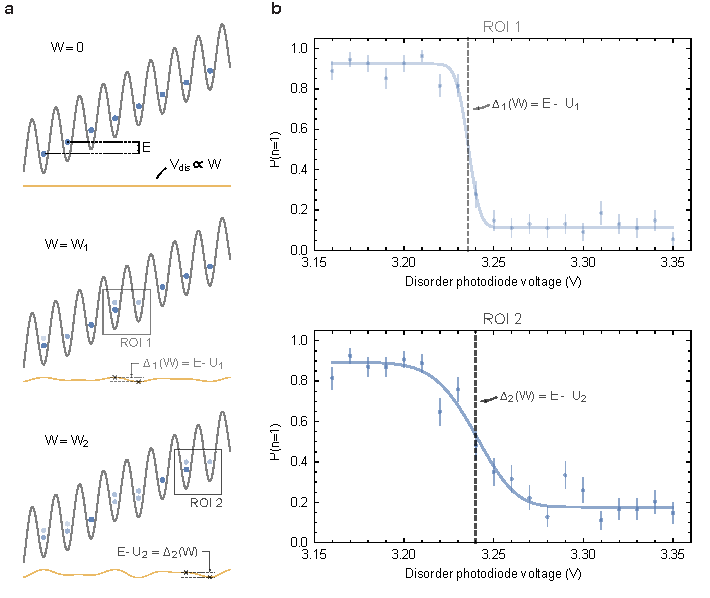
\includegraphics[width=\columnwidth]{figures/ch2/disorder_cal/Wcalv2edit.pdf} 
%		\caption{\textbf{Calibration of on-site potential offsets ($h_i$). a)} This illustration demonstrates the protocol for finding the on-site potential offset by adiabatic passage of an atom onto its neighbor. \textbf{b)} By finding the crossing point of these Landau-Zener like crossings, we are able to fit the resonance crossing to extract the local potential offset between neighboring sites.}
%		\label{fig:WCal}	
%\end{figure}

\begin{figure}
\floatbox[{\capbeside\thisfloatsetup{capbesideposition={right,top},capbesidewidth=1.5 in}}]{figure}[\FBwidth]
{\caption{\textbf{Calibration of on-site potential offsets ($h_i$). a)} This illustration demonstrates the protocol for finding the on-site potential offset by adiabatic passage of an atom onto its neighbor. \textbf{b)} By finding the crossing point of these Landau-Zener like crossings, we are able to fit the resonance crossing to extract the local potential offset between neighboring sites. Note that the $x$-axis is the voltage on the photodiode that is logarithmically sensitive to the power in the beam with $0.5\text{V/decade}$ as the calibrated slope.}
		\label{fig:WCal}	}
{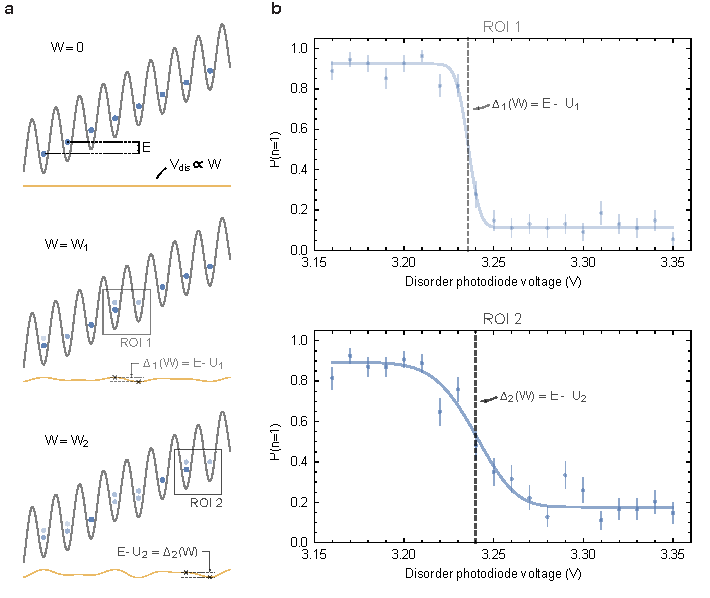
\includegraphics[width=4 in]{figures/ch2/disorder_cal/Wcalv2edit.pdf} }
\end{figure}

We used a similar protocol to the $U$ calibration method mentioned above in \S \ref{sec:EUcal} and is a hybrid of the protocols used in previous studies \cite{Ma2011,Simon2011}. The method starts with a unity-filled Mott-insulating state. A tilt of strength $E$ Hz/site is then applied to the system to bring all sites far from resonance with their neighbors. The lattice depth is then reduced to an intermediate depth with appreciable but small tunneling. The additional potential pattern is then turned on approximately adiabatically with respect to only the nearest neighbor tunneling strength $J$. Since the potential that is applied has varying on-site potentials $h_i$, the resonance condition is again re-established when the energy difference between neighboring sites, $\Delta_i = h_i - h_{i-1}$, compensates for the energy offset $E-U$. The signal for this transition is finding when the average on-site occupation changes from $n=1$ atom to $n=0,2$. This is actually measured in-situ as a change in parity. The example for this method shown in Fig.~\ref{fig:WCal} is performed for an on-site potential sampled from a quasi-periodic distribution: $h_i = W \cos{\left (  2 \pi \beta i + \phi_o \right ) }$, where $\beta$ is the golden ratio $\approx 1.618$, $i$ is the site-index, and $\phi_o$ is an arbitrary phase factor. This protocol is also described in the supplementary information of \emph{Lukin et al.}\cite{Lukin2019}.

\subsection{Heating rates : spontaneous scattering}

As discussed earlier in \S \ref{sec:ch2_heating}, the spontaneous scattering rate provides a limit on the lifetime of many-body coherent processes. To estimate this limit, we determine the contribution of the spontaneous scattering rates present from all the confining optical potentials in the system. The approximate background lifetime related to background collisions with hot atoms (this is related to the vacuum quality in the glass cell) is a lifetime of $\tau_{Bkg} = 33(3)\mathrm{s}$ or scattering rate $\gamma_{Bkg} = 0.03(3)\mathrm{Hz}$. By measuring the atom loss rate from relatively weak traps as a function of optical potential depth, we can measure the contribution of the additional optical potential to heating and the offset that comes from background gas collisions. In general, this loss will follow an exponential form $\sim n(t) = N_o e^{-\gamma_{Bkg} t - \gamma_{Optical}(V_o) t}$. By holding the atoms in just an optical harmonic potential (a large Laguerre-Gauss beam) and the axial confinement lattice, we were able to find good agreement with the predicted spontaneous scattering rate and the approximate background collision rate estimated by previous works (Fig.~\ref{fig:heatingCal})\cite{Gillen2009,Bakr2011,Preiss2015}. These measurements put an approximate single-atom lifetime bound due to the combination of all decay mechanisms in the experiments presented in this thesis to be $\tau_{all+axial} \approx 14\mathrm{s}$ in the axial-lattice configuration and $\tau_{all+big} \approx 19$s in the big-lattice configuration.

\begin{figure}[t!]
		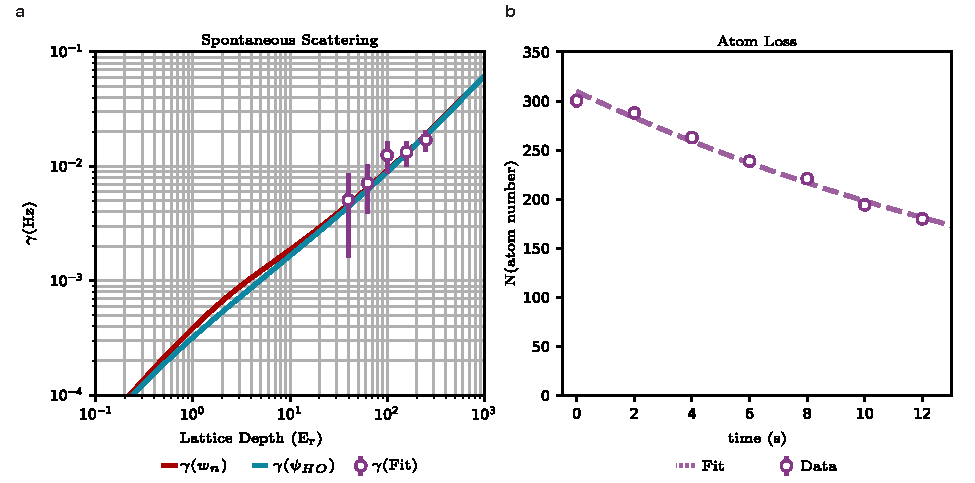
\includegraphics[width=\columnwidth]{figures/ch2/heating_rates/ScatteringRatesCalv2v2edit.pdf} 
		\caption{\textbf{Axial lattice heating rate. a)} The plotted data points are determined directly from the fit of an exponential decay to the atom loss from the optical trap at various axial lattice depths after removing the static contribution from the background lifetime independent of lattice depth. \textbf{b)} The atom loss from the optical trap as a function of time. The dashed line represents the fitted exponential decay.}
		\label{fig:heatingCal}	
\end{figure}


%\subsection{MI to SF heating? \textcolor{red}{THINK ABOUT THIS LATER}}

